\tikzstyle{input_neuron}=[circle,draw=red!50,fill=red!10,thick,minimum size=6mm]
\tikzstyle{hidden_neuron}=[circle,draw=blue!50,fill=cyan!10,thick,minimum size=6mm]
\tikzstyle{output_neuron}=[circle,draw=green!50,fill=green!10,thick,minimum size=6mm]
\tikzstyle{cpy_neuron}=[circle,draw=red!50,fill=red!50,thick,minimum size=6mm]
\tikzstyle{input}=[circle,draw=black!50,fill=black!20,thick,minimum size=6mm]

\begin{center}
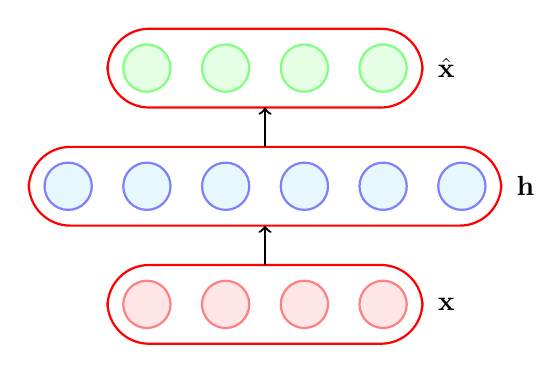
\begin{tikzpicture}

\node [input_neuron] (neuron01) at (8.5,4.5) {};
\node [input_neuron] (neuron02) at (9.5,4.5){};
\node [input_neuron] (neuron03) at (10.5,4.5) {};
\node [input_neuron] (neuron04) at (11.5,4.5) {};
\node [hidden_neuron] (neuron51) at (7.5,6) {} ;
\node [hidden_neuron] (neuron52) at (8.5,6)  {};
\node [hidden_neuron] (neuron53) at (9.5,6)  {};
\node [hidden_neuron] (neuron54) at (10.5,6)  {};
\node [hidden_neuron] (neuron55) at (11.5,6)  {};
\node [hidden_neuron] (neuron56) at (12.5,6)  {};

\node [output_neuron] (neuron11) at (8.5,7.5)  {};
\node [output_neuron] (neuron12) at (9.5,7.5)  {};
\node [output_neuron] (neuron13) at (10.5,7.5)  {};
\node [output_neuron] (neuron14) at (11.5,7.5)  {};


\node[text width=0.01cm] at (12.2,4.5) {$\textbf{x}$};
\node[text width=0.01cm] at (13.2,6) {$\textbf{h}$};
\node[text width=0.01cm] at (12.2,7.5) {$\hat{\textbf{x}}$};

\draw[red!100,thick,solid,rounded corners=15pt] (8,4) rectangle (12,5);
\draw[red!100,thick,solid,rounded corners=15pt] (7,5.5) rectangle (13,6.5);
\draw[red!100,thick,solid,rounded corners=15pt] (8,7) rectangle (12,8);


\draw[thick,->] (10,5) -- (10,5.5);

\draw[thick,->] (10,6.5) -- (10,7);

\end{tikzpicture}
\end{center}